\section{Variedades Diferenciables}

\begin{definition}
Una \textit{\textbf{variedad diferenciable}} de dimensi\'on $n$ es un conjunto $M$ dotado de una familia de mapeos 1:1
\begin{equation*}
    \mathbf{x}_\alpha\colon U_\alpha\subseteq\mathbb{R}^n\to M,\quad\alpha\in A
\end{equation*}
tales que
\begin{enumerate}
    \item[(i)] $\displaystyle{\bigcup_{\alpha\in A}\mathbf{x}_\alpha(U_\alpha)=M}$.
    \item[(ii)] $\forall\alpha,\beta$ con $\mathbf{x}_\alpha(U_\alpha)\cap\mathbf{x}_\beta(U_\beta)=W\neq\varnothing$, el mapa $\mathbf{x}_\beta^{-1}\circ\mathbf{x}_\alpha\colon\mathbf{x}_\alpha^{-1}(W)\subseteq\mathbb{R}^n\to\mathbf{x}_\beta^{-1}(W)\subseteq\mathbb{R}^n$ es diferenciable.
\end{enumerate}
\end{definition}
\begin{definition}
A los mapeos $\mathbf{x}_\alpha$ les llamamos \textit{\textbf{parametrizaciones}} o \textit{\textbf{sistema de coordenadas}}.   
\end{definition}

\begin{example}
$\mathbb{S}^2=\{(x,y,z)\in\mathbb{R}^3\colon x^2+y^2+z^2=1\}$. Sean $N=(0,0,1)$ y $S=(0,0,-1)$. Definimos
\begin{align*}
    &\pi^N\colon\mathbb{S}^2\backslash\{N\}\to\mathbb{R}^2\\
    &(x,y,z)\mapsto\left(u=\frac{x}{1-z},v=\frac{y}{1-z}\right).
\end{align*}
Entonces $\bigl(\mathbb{S}^2,\alpha^N=(\pi^N)^{-1},\alpha^S=(\pi^S)^{-1}\bigl)$ es una variedad diferenciable de dimensi\'on 2. Se puede probar que, en la intersecci\'on $W=\mathbb{S}^2\backslash\{N\}\cup\{S\}$ tenemos 
\begin{equation*}
    u'=\frac{u}{u^2+v^2},\quad v'=\frac{v}{u^2+v^2}.
\end{equation*}
\end{example}

\begin{definition}
A las funciones $\mathbf{x}_\alpha^{-1}\circ\mathbf{x}_\beta\colon\mathbb{R}^n\to\mathbb{R}^n$ les llamamos \textit{\textbf{cambio de coordenadas}} o \textit{\textbf{cambio de par\'ametro}}.    
\end{definition}
A continuaci\'on, podemos ver un esquema de c\'omo se podr\'ia representar, por definici\'on, una variedad diferenciable.
\begin{figure}[ht]
    \caption{Ilustraci\'on de una Variedad Diferenciable}
    \centering
    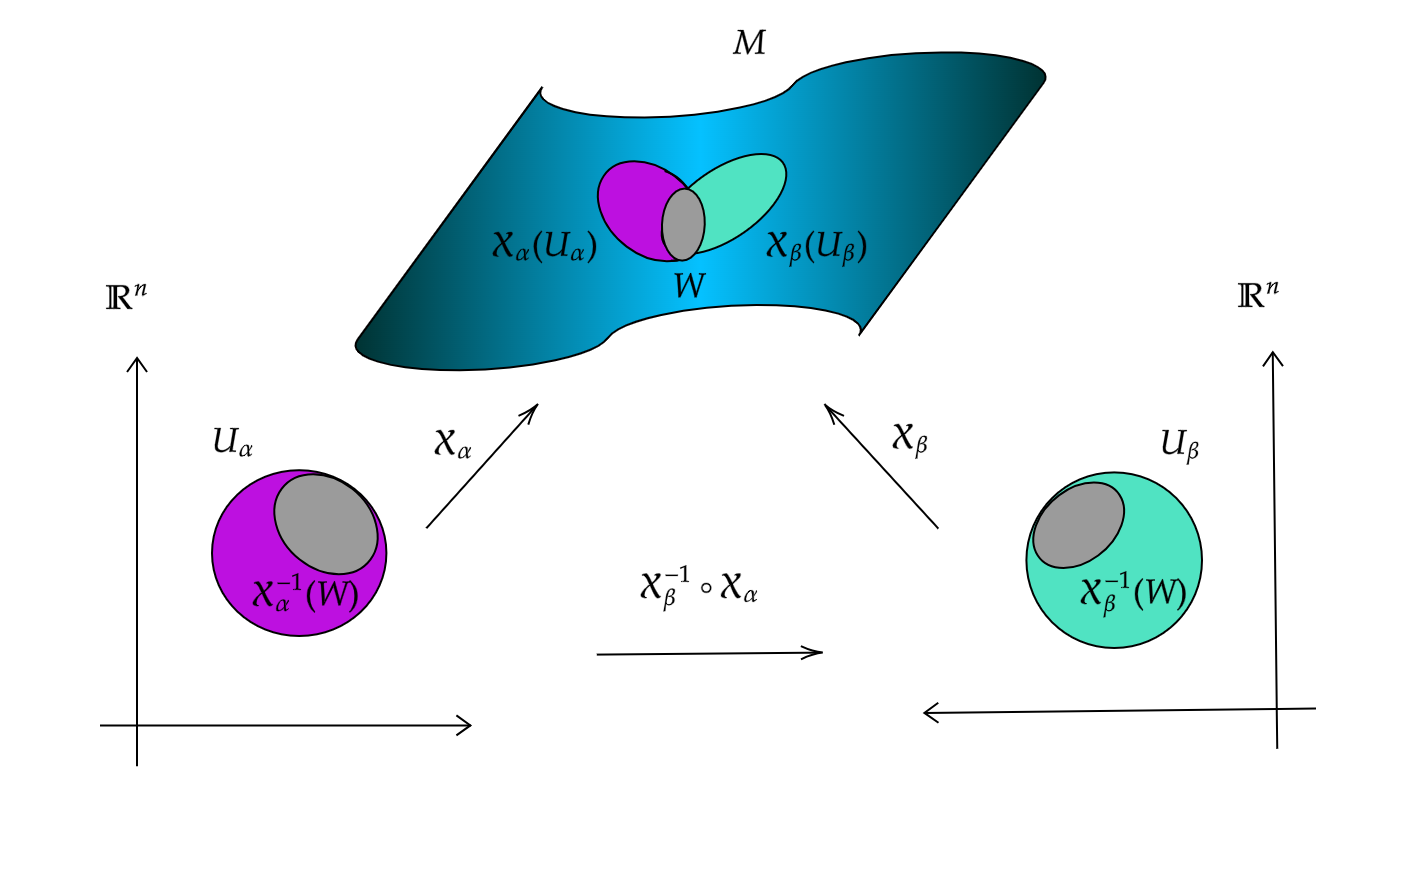
\includegraphics[width=\textwidth]{capitulos/variedaddif.png}
\end{figure}
\section{Funciones Diferenciables}

\begin{definition}
Dada $\varphi\colon M_1^n\to M_2^m$ se dice \textit{\textbf{diferenciable}} en $p\in M_1^n$ si, dada una parametrizaci\'on $\mathbf{y}$ de mi entorno de $\varphi(p)$, existe una parametrizaci\'on $\mathbf{x}$ de un entorno $U$ de $p$ tal que
\begin{equation*}
    \hat{\varphi}_{\mathbf{xy}}:=\mathbf{y}^{-1}\circ\varphi\circ\mathbf{x}\colon U\subseteq\mathbb{R}^n\to\mathbb{R}^m
\end{equation*}
sea diferenciable.
\end{definition}

\begin{theorem}
La definici\'on de diferenciabilidad est\'a bien dada (no depende de la elecci\'on de $\mathbf{x}$,$\mathbf{y}$).
\end{theorem}
\begin{proof}[\textbf{Demostraci\'on}]
Necesitamos demostrar que $\hat{\varphi}_{\mathbf{xy}}\in C^{\infty}$ si y solo si $\hat{\varphi}_{\tilde{\mathbf{x}}\tilde{\mathbf{y}}}$.
Para ello, notemos que 
\begin{align*}
    \hat{\varphi}_{\mathbf{xy}}&=\mathbf{y}^{-1}\circ\varphi\circ\mathbf{x}\\
    &=\underbrace{\mathbf{y}^{-1}\circ\tilde{\mathbf{y}}}_{C^\infty}\circ\underbrace{\tilde{\mathbf{y}}^{-1}\circ\varphi\circ\tilde{\mathbf{x}}}_{\hat{\varphi}_{\tilde{\mathbf{x}}\tilde{\mathbf{y}}}}\circ\underbrace{\tilde{\mathbf{x}}^{-1}\circ\mathbf{x}}_{C^\infty}.
\end{align*}
Notemos que, la igualdad anterior demuestra que $\hat{\varphi}_{\mathbf{xy}}\in C^{\infty}$ si y solo si $\hat{\varphi}_{\tilde{\mathbf{x}}\tilde{\mathbf{y}}}\in C^{\infty}$.
\end{proof}

\begin{definition}
$\hat{\varphi}_{\mathbf{xy}}$ se llama \textit{\textbf{representaci\'on en coordenadas}} de $\varphi$.    
\end{definition}

\begin{notation}
Cuando se escriba
\begin{equation*}
    \varphi(x^1,\dots,x^n)=\Bigl(\varphi^1(x^1,\dots,x^n),\dots,\varphi^m(x^1,\dots,x^n)\Bigl),
\end{equation*}
se entender\'a entonces que
\begin{equation*}
    \hat{\varphi}_{\mathbf{xy}}(x^1,\dots,x^n)=\Bigl(\hat{\varphi}_{\mathbf{xy}}^1(x^1,\dots,x^n),\dots,\hat{\varphi}_{\mathbf{xy}}^m(x^1,\dots,x^n)\Bigl).
\end{equation*}
\end{notation}

\begin{definition}
Decimos que $f\colon M_1\to M_2$ es un \textit{\textbf{difeomorfismo}} si $f\in C^\infty$ y si existe $f^{-1}$ tal que $f^{-1}\in C^\infty$   
\end{definition}

\begin{observation}
Regresando a las preguntas de la secci\'on 6.3, dados los modelos:
    \begin{enumerate}[label=(\alph*)]
        \item $p_1(x;\theta)=p(x;\mu,\sigma)=\frac{1}{\sqrt{2\pi}\sigma}e^{-\frac{1}{2}\frac{(x-\mu)^2}{\sigma^2}},\quad x\in\mathbb{R}\text{ y }(\mu,\sigma)\in\mathbb{R}\times\mathbb{R}_+$
        \item $p_2(x;\eta)=p(x;\rho,\tau)=\frac{\tau}{\sqrt{2\pi}}e^{-\frac{1}{2}(x\tau-\rho\tau+1)^2},\quad x\in\mathbb{R}\text{ y }(\rho,\tau)\in\mathbb{R}\times\mathbb{R}_+$\\
        y con $\rho=\mu+\sigma$, $\tau=\frac{1}{\sigma}$.
    \end{enumerate}
¿Podemos afirmar que $p_1(x;\theta)=p_2(x;\eta)$?\\

\noindent\textbf{S\'I:} Utilizando la definici\'on de difeomorfismo, podemos decir que $p_1(x;\theta)=p_2(x;\eta)$ pues definen la misma variedad, 
siendo $\eta_1=\theta_1+\theta_2=\mu+\sigma$ y $\eta_2=1/\theta_2=1/\sigma$ es cambio de coordenadas correspondiente.
%pero una funci\'on es el cambio de coordenadas para la otra. 
\end{observation}

\section{El Espacio Tangente}
\begin{definition}[\textbf{Tentativa}]
Decimos que $w\in T_pM$ si existe $\gamma\colon(-\varepsilon,\varepsilon)\to M$ tal que $\gamma(0)=p$ y  $\gamma'(0)=w$, donde $T_pM$ representa el espacio tangente a $M$ en $p\in M$.   
\end{definition}

\begin{observation}
La definici\'on anterior no nos funciona por el momento, pues con la informaci\'on que tenemos, no podemos calcular $\gamma'(0)$.    
\end{observation}

\subsection*{Motivaci\'on para una Definici\'on Formal:}

\noindent En $\mathbb{R}^n$, tomemos la curva 
\begin{equation*}
    \gamma\colon(-\varepsilon,\varepsilon)\to\mathbb{R}^n
\end{equation*}
la cual, cumple que
\begin{align*}
    \gamma(0)&=(x^1(0),\dots,x^n(0))=p\\
    \gamma'(0)&=\Bigl((x^1)'(0),\dots,(x^n)'(0)\Bigl)=w.
\end{align*}
Ahora, si tomamos $f\colon U_p\subseteq\mathbb{R}^n\to\mathbb{R}$, podemos definir la \textit{\textbf{derivada direccional}} de la siguiente manera:
\begin{align*}
    w_p(f)=df_p(w)&=\frac{d}{dt}f\circ\gamma\Big|_{t=0}\\
    &=\frac{\partial f}{\partial x^i}\Big|_p(x^i)'(0)\\
    &=\underbrace{(x^i)'(0)\frac{\partial}{\partial x^i}}_{w_p}f\Big|_p.
\end{align*}
Notemos que esta propiedad es intr\'inseca, pues solo necesito definir coordenadas a partir de la variedad diferencial en la que estamos. Esta idea motiva a definir lo siguiente:

\begin{definition}
Sea $M$ una variedad diferenciable y $\gamma\colon(-\varepsilon,\varepsilon)\to M$ tal que $\gamma(0)=p$. Sea 
\begin{equation*}
    D_p=\{f\colon M\to\mathbb{R}\colon\text{$f$ es difernciable en $p$}\}.
\end{equation*}
Definimos el \textit{\textbf{vector tangente}} a $\gamma$ en $p$ (con $t=0$), como la funci\'on
\begin{equation*}
    \gamma'(0)\colon D_p\to\mathbb{R}
\end{equation*}
dada por 
\begin{equation*}
    \gamma'(0)(f)=\frac{d}{dt}f\circ\gamma\Big|_{t=0}.
\end{equation*}
Por lo tanto, $w$ un \textit{\textbf{vector tangente}} a $M$ en $p$, es un vector tangente a $\gamma$ en $t=0$ por alguna $\gamma\colon(-\varepsilon,\varepsilon)\to M$ tal que $\gamma(0)=p$.
\end{definition}

\begin{notation}
En coordenadas, expresaremos 
\begin{equation}
    w(f)=\underbrace{(x^i)'(0)}_{\gamma'(0)}\frac{\partial}{\partial x^i}f\Big|_{p=\gamma(0)}
\end{equation}
donde $\mathbf{x}\colon U\subseteq\mathbb{R}^n\to U_p\subseteq M$ es la parametrizaci\'on.
\end{notation}

\begin{observation}
Dada la notaci\'on anterior, tenemos las siguientes observaciones:
\begin{enumerate}[label=(\alph*)]
    \item Para la ecuaci\'on (7.1), si $w=\frac{\partial}{\partial x^i}$, entonces $w$ es tangente a la \textit{\textbf{curva coordenada}} $x^i$.
    \item Por la ecuaci\'on (7.1), vemos que la definici\'on de $w$ s\'olo depende de $\gamma(0)$ y $\gamma'(0)$.
    \item El espacio de todos los vectores tangentes a $M$ en $p$ llamado \textit{\textbf{espacio tangente}} a $M$ en $p$, indicado con $T_pM$, es un espacio vectorial de dimensi\'on $n$ y adem\'as ya conocemos la base coordenada $\{\frac{\partial}{\partial x^i}|_p\}$ conocida como la base asociada a la parametrizaci\'on $\mathbf{x}$.
\end{enumerate}    
\end{observation}

\section{Diferencial y Campos Vectoriales}

\begin{definition}
Sea $\varphi\colon M_1\to M_2$ y sean $p\in M_1$ y $v\in T_pM$. Definimos el \textit{\textbf{diferencial}} de $\varphi$ en $p$ como la funci\'on 
\begin{equation*}
    d\varphi_p\colon T_pM_1\to T_{\varphi(p)}M_2
\end{equation*}
dada por
\begin{equation*}
    d\varphi_p(v)=\frac{d}{dt}\varphi\circ\gamma\Big|_{t=0}
\end{equation*}
donde $\gamma$ es una curva tal que $\gamma(0)=p$ y $\gamma'(0)=v$.
\end{definition}

\begin{theorem}
El diferencial $d\varphi_p$ cumple las siguientes propiedades:
\begin{enumerate}
    \item[(i)] Es lineal,
    \item[(ii)] No depende de la elecci\'on de $\gamma$ en la clase $[\gamma]=v$. 
\end{enumerate}
\end{theorem}
\begin{proof}[\textbf{Idea para la Demostraci\'on}]
Tomemos la ecuaci\'on 
\begin{equation}
    d\varphi_p(v)=\frac{\partial\varphi^i}{\partial x^j}\Big|_p(x^j)'(0)=\mathbf{J}\varphi_p\cdot[v]
\end{equation}
donde 
\begin{equation*}
    [v]=\Bigl((x^1)'(0)\dots,(x^n)'(0)\Bigl).
\end{equation*}
\end{proof}

\begin{definition}
Un \textit{\textbf{campo vectorial}} $\mathbf{X}$ sobre $M$ es una funci\'on que asocia a todo punto $p\in M$ un vector tangente $\mathbf{X}(p)$ a $M$ en $p$.    
\end{definition}

\begin{definition}
Se llama \textit{\textbf{haz tangente}} de $M$ la variedad diferenciable de dimensi\'on $2n$ dada por 
\begin{equation*}
    TM=\bigcup_{p\in M}T_pM.
\end{equation*}
\end{definition}

\begin{observation}
En coordenadas, se tiene que $\mathbf{X}(p)=\mathbf{X}^i(p)\frac{\partial}{\partial x^i}$. Entonces,
\begin{equation}
    \mathbf{X}(p)(f)=\mathbf{X}^i(p)\frac{\partial}{\partial x^i}f=df_p(\mathbf{X}).
\end{equation}
\end{observation}

\begin{definition}
Dado $\mathbf{X}\in\mathfrak{X}(M)$, $\gamma$ se llama \textit{\textbf{curva integral}} (\textit{\textbf{trayectoria}}) de $\mathbf{X}$ si 
\begin{equation}
    \gamma'(t)=\mathbf{X}(\gamma(t)),\quad\forall t\in(-\varepsilon,\varepsilon)
\end{equation}
En coordenadas, se representa como:
\begin{align*}
    &\gamma(t)=\Bigl(x^1(t),\dots,x^n(t)\Bigl)\\
    \text{Sistema de E.D.O's}
    &\begin{cases}
    (x^1)'(t)=\mathbf{X}^1\Bigl(x^1(t),\dots,x^n(t)\Bigl)\\
    \vdots\\
    (x^n)'(t)=\mathbf{X}^n\Bigl(x^1(t),\dots,x^n(t)\Bigl)
    \end{cases}\\
    \text{Condici\'on Inicial: }
    &\gamma(0)=q\overset{\text{En coord.}}{\iff}x^i(0)=x_0^i
\end{align*}
\end{definition}

\begin{theorem}[\textbf{Existencia y Unicidad de Curvas Integrales}]
Dada $\mathbf{X}\in\mathfrak{X}(M)$ y dada $q\in M$ existe una \'unica curva $\gamma\colon(-\varepsilon,\varepsilon)\to M$ tal que $\gamma$ es la curva integral de $\mathbf{X}$ que pasa por $p$.    
\end{theorem}

%\begin{observation}[\textbf{Convenci\'on de Einstein}]
%Recordemos que seg\'un la Ecuaci\'on (7.3), dado $\mathbf{X}\in\mathfrak{X}(M)$, la convenci\'on de Einstein estar\'a expresada por
%\begin{align*}
%    \mathbf{X}_p(f)=\mathbf{X}^i(x)\frac{\partial}{\partial x^i}f\Big|_p=df_p(\mathbf{X}),\quad i\in\{1,2,\dots,n\}.
%\end{align*}
%En la siguiente secci\'on, daremos una generalizaci\'on de esta idea.
%\end{observation}

\section{Tensores}

\begin{observation}
En la secci\'on anterior, vimos que dada una variedad diferenciable $M$ y dado $p\in M$, 
$T_pM$ es un espacio vectorial de dimensi\'on $n$. Seguiremos esta misma idea para escribir la siguente definici\'on.   
\end{observation}

\begin{definition}
Llamamos \textit{\textbf{espacio cotangente}} de $M$ en $p$ al conjunto dado por 
\begin{align*}
    T_p^{*}M=(T_pM)^{*}=\{f\colon T_pM\to\mathbb{R}|\text{$f$ es lineal}\}
\end{align*}
Sus elementos se llaman \textit{\textbf{covectores}} o \textit{\textbf{1-formas}}.
\end{definition}

\begin{example}
Sea $f\colon M\to\mathbb{R}$ tal que $f\in C^\infty$. Entonces $df_p\colon T_pM\to\mathbb{R}$ es lineal. De esta manera, $df_p\in T_p^{*}M$. En particular, si $\mathbf{x}\colon U\subseteq\mathbb{R}^n\to M$ es una parametrizaci\'on, se tendr\'a que $dx^i\in T_p^{*}M$.   

Resulta que $\{dx_p^i\}_{i=1}^{n}$ es una \textit{\textbf{base coordenada}} de $T_p^{*}M$ y adem\'as es la base dual de $\{\frac{\partial}{\partial x^j}|_p\}$ en el sentido de que, por la Ecuaci\'on (7.3), se tiene que 
\begin{equation*}
    dx^i\left(\frac{\partial}{\partial x^j}\right)=\frac{\partial}{\partial x^j}(x^i)=\delta_j^i.
\end{equation*}
\end{example}

\begin{definition}
Decimos que 
\begin{equation*}
    T^*M:=\bigcup_{p\in M}T_p^{*}M 
\end{equation*}
se llama el \textit{\textbf{haz cotangente}} de $M$ y es una variedad diferenciable de dimensi\'on $2n$ 
(con coordenadas locales $(x^i,\alpha_i)$).
\end{definition}

\begin{observation}
En general, una 1-forma $\alpha$ la puedo escribir en coordenadas como:
\begin{equation*}
    \alpha=\alpha_idx^i
\end{equation*}
\end{observation}

\begin{observation}
Dado un espacio vectorial $V$ finito-dimensional, sabemos que $(V^*)^*=V$. Esto nos dice que 
\begin{equation*}
    T_pM=\{f\colon T_p^{*}M\to\mathbb{R}\text{ lineales }\}.
\end{equation*}
\end{observation}

\begin{definition}
Decimos que 
\begin{equation*}
    \mathcal{T}_p^{(r,s)}M:=\Biggl\{f\colon\underbrace{T_p^{*}M\times\cdots\times T_p^{*}M}_{\text{$r$-veces}}\times\underbrace{T_pM\times\cdots\times T_pM}_{\text{$s$-veces}}\to\mathbb{R}\Bigg|\text{$f$ es lineal}\Biggl\}
\end{equation*}
se llama \textit{\textbf{espacio de los tensores}} de tipo $(r,s)$ de $M$ en $p$. Sus elementos se llaman \textit{\textbf{tensores}} de tipo $(r,s)$ en $p$.
\end{definition}

\begin{example}
Dada la definici\'on anterior, obtenemos las siguientes observaciones:
\begin{enumerate}
    \item[(i)] Los vectores de $T_pM$ son tensores de tipo $(1,0)$.
    \item[(ii)] Los covectores son tensores de tipo $(0,1)$ (1-formas).
\end{enumerate}
\end{example}

\begin{definition}
La variedad diferenciable 
\begin{equation*}
    \mathcal{T}^{(r,s)}:=\bigcup_{p\in M}\mathcal{T}_p^{(r,s)}M
\end{equation*}
se llama \textit{\textbf{haz de los tensores}} de tipo $(r,s)$.
\end{definition}

\begin{definition}
Dado $A\in\mathcal{T}^{(n,m)}M$ y $B\in\mathcal{T}^{(r,s)}M$, se define el \textit{\textbf{producto tensorial}} de $A$ y $B$ como el tensor 
\begin{equation*}
    A\otimes B\in\mathcal{T}^{(n+r,m+s)}M
\end{equation*}
dado por 
\begin{align*}
    &A\otimes B(\alpha_1,\dots,\alpha_{n+r},v_1,\dots,v_{m+s})\\
    &:=A(\alpha_1,\dots,\alpha_n,v_1,\dots,v_m)B(\alpha_{n+1},\dots,\alpha_{n+r},v_{m+1},\dots,v_{m+s}).
\end{align*}
\end{definition}

\begin{observation}
Dada $\mathbf{x}\colon U\subseteq\mathbb{R}^n\to M$ parametrizaci\'on, tenemos la \textit{\textbf{base coordenada}} (\textit{\textbf{base asociada}}) de $\mathcal{T}_p^{(r,s)}M$ dada por
\begin{equation*}
    \frac{\partial}{\partial x^{i_1}}\otimes\cdots\otimes\frac{\partial}{\partial x^{i_n}}\otimes dx^{j_1}\otimes\cdots\otimes dx^{j_s}
\end{equation*}
para 
\begin{align*}
    i_1&=1,\dots,n\\
    &\vdots\\
    i_r&=1,\dots,n\\
    j_1&=1,\dots,n\\
    &\vdots\\
    j_s&=1,\dots,n.
\end{align*}
En general, un tensor $\tau\in\mathcal{T}_p^{(r,s)}M$ se va a ver como 
\begin{align*}
    \tau=\tau^{i_1\dots i_n}_{j_1\dots j_s}    \frac{\partial}{\partial x^{i_1}}\otimes\cdots\otimes\frac{\partial}{\partial x^{i_n}}\otimes dx^{j_1}\otimes\cdots\otimes dx^{j_s}
\end{align*}
donde $\tau^{i_1\dots i_n}_{j_1\dots j_s}$ es la componente de $\tau$ en la base coordenada de $\mathcal{T}_p^{(r,s)}M$.
\end{observation}

\begin{example}
De los conceptos anteriores, podemos obtener los siguientes ejemplos:
\begin{enumerate}
    \item[(i)] Si $v$ es un tensor de tipo $(1,0)$, entonces
    \begin{equation*}
        v=v^i\frac{\partial}{\partial x^i},\quad([v]^i=v^i).
    \end{equation*}
    \item[(ii)] Si $\alpha$ es una tensor de tipo $(0,1)$, entonces
    \begin{equation*}
        \alpha=\alpha_idx^i,\quad([\alpha]_i=\alpha_i).
    \end{equation*}
    \item[(iii)] Si $g$ es un tensor de tipo (0,2), entonces
    \begin{equation*}
        g=g_{ij}dx^i\otimes dx^j,\quad([g]_{ij}=g_{ij}).
    \end{equation*}
\end{enumerate}
\end{example}

\begin{observation}[\textbf{Importante}]
Con la informaci\'on anterior, podemos hacer las siguientes preguntas:
\begin{enumerate}
    \item[(i)] ¿C\'omo calcular las componentes de un tensor en una base?
    \item[(ii)] ¿C\'omo cambian las componentes al cambiar de base?
\end{enumerate}
\end{observation}

\noindent\textbf{Respuestas:}
\begin{itemize}
    \item Para $v$ de tipo $(1,0)$, se tiene en coordenadas que
    \begin{equation*}
        v=v^i\frac{\partial}{\partial x^i}.
    \end{equation*}
    \begin{enumerate}
        \item[(i)] $v^i=v(x^i)\quad\|\quad\tilde{v}^j=v(\tilde{x}^j)$.
        \item[(ii)] Se tiene la siguiente ecuaci\'on:
        \begin{equation}
            \tilde{v}^j=v^i\frac{\partial}{\partial x^i}(\tilde{x}^j)=\frac{\partial\tilde{x}^j}{\partial x^i}v^i.
        \end{equation}
    \end{enumerate}
    Se dice que un tensor de tipo $(1,0)$ tiene 1 \textit{\textbf{\'indice contravariante}}.
    \item Para $\alpha$ de tipo $(0,1)$, se tiene en coordenadas que 
    \begin{equation*}
        \alpha=\alpha_idx^i.
    \end{equation*}
    \begin{enumerate}
        \item[(i)] $\alpha_i=\alpha\left(\frac{\partial}{\partial x^i}\right)\quad\|\quad\tilde{\alpha}_j=\alpha\left(\frac{\partial}{\partial\tilde{x}^j}\right)$.
        \item[(ii)] Se tiene la siguiente ecuaci\'on:
        \begin{equation}
            \tilde{\alpha}_j=\alpha_idx^i\left(\frac{\partial}{\partial\tilde{x}^j}\right)=\frac{\partial x^i}{\partial\tilde{x}^j}\alpha_i.
        \end{equation}
    \end{enumerate}
     Se dice que un tensor de tipo $(0,1)$ tiene 1 \textit{\textbf{\'indice covariante}}.
     \item Para $g$ de tipo $(0,2)$ se tiene en coordenadas que 
     \begin{equation*}
         g=g_{ij}dx^i\otimes dx^j.
     \end{equation*}
     \begin{enumerate}
         \item[(i)] $g_{ij}=g\left(\frac{\partial}{\partial x^i},\frac{\partial}{\partial x^j}\right)\quad\|\quad\tilde{g}_{rs}=g\left(\frac{\partial}{\partial\tilde{x}^r},\frac{\partial}{\partial\tilde{x}^s}\right)$.
         \item[(ii)] Se tiene la siguiente ecuaci\'on:
         \begin{equation}
             \tilde{g}_{rs}=g\left(\frac{\partial}{\partial\tilde{x}^r},\frac{\partial}{\partial\tilde{x}^s}\right)=g_{ij}dx^i\otimes dx^j\left(\frac{\partial}{\partial\tilde{x}^r},\frac{\partial}{\partial\tilde{x}^s}\right)=g_{ij}\frac{\partial x^i}{\partial\tilde{x}^r}\frac{\partial x^j}{\partial\tilde{x}^s}.
         \end{equation}
     \end{enumerate}
          Se dice que un tensor de tipo $(0,2)$ tiene 2 \textit{\textbf{\'indices covariantes}}.
\end{itemize}

\begin{observation}
A las ecuaciones (7.5), (7.6) y (7.7) las podemos ver como definiciones de tensor.   
\end{observation}

\begin{example}
Dada $f\colon M\to\mathbb{R}$ y dada $\mathbf{x}\colon U\subseteq\mathbb{R}^n\to M$ parametrizaci\'on, podemos definir $\partial f$ cuyas componentes en la base coordenada son
\begin{equation*}
    [\partial f]=\left(\frac{\partial f}{\partial x^1},\dots,\frac{\partial f}{\partial x^n}\right)
\end{equation*}
 y me pregunto si son las componentes de alg\'un tensor, por ejemplo, si son las componentes de un campo vectorial (el gradiente de $f$).
\end{example}

\begin{theorem}
La definici\'on de $\partial f$, cumple los siguientes incisos:
\begin{enumerate}[label=(\alph*)]
    \item No es un campo vectorial.
    \item Es una 1-forma.
    \item $\partial f=df$
\end{enumerate}
\end{theorem}
\begin{proof}[\textbf{Demostraci\'on}]
\begin{enumerate}[label=(\alph*)]
    \item Por definici\'on, se tiene que 
    \begin{equation*}
        v^i=\frac{\partial f}{\partial x^i}\quad\|\quad\tilde{v}^j=\frac{\partial f}{\partial\tilde{x}^j}
    \end{equation*}
    pero 
    \begin{equation*}
        \tilde{v}^i=\frac{\partial f}{\partial\tilde{x}^i}=\frac{\partial x^j}{\partial\tilde{x}^i}\frac{\partial f}{\partial x^j}=\frac{\partial x^j}{\partial\tilde{x}^i}v^j
    \end{equation*}
    \item Notemos que
    \begin{equation*}
        \alpha_i=\frac{\partial f}{\partial x^i}\quad\text{y}\quad\tilde{\alpha}_i=\frac{\partial x^j}{\partial\tilde{x}^i}\alpha_j
    \end{equation*}
    \item Por \'ultimo, observemos que 
    \begin{equation*}
        (\partial f)_i=\frac{\partial f}{\partial x^i}=\alpha_i
    \end{equation*}
    lo cual, implica que
    \begin{equation*}
        \alpha=\partial f=\frac{\partial f}{\partial x^i}dx^i=df.
    \end{equation*}
\end{enumerate}    
\end{proof}

\section{M\'etricas Riemannianas}

\begin{definition}
Una \textit{\textbf{m\'etrica riemanniana}} en $M$ es un campo tensorial $g$ de tipo $(0,2)$ tal que $\forall p\in M$, $g_p$ 
es un producto escalar euclideano en $T_pM$ (bilineal, sim\'etrico y definido positivo).
\end{definition}

\begin{notation}
La definici\'on anterior justifica la siguiente notaci\'on:
\begin{align*}
    g_p(v_1,v_2)&=\langle v_1,v_2\rangle\\
    g(\mathbf{X},\mathbf{Y})&=\langle \mathbf{X},\mathbf{Y}\rangle.
\end{align*}
\end{notation}

\noindent\textbf{En Coordenadas:} Sean 
\begin{equation*}
    g_{ij}(x)=g\left(\frac{\partial}{\partial x^i},\frac{\partial}{\partial x^j}\right)
\end{equation*}
y sean
\begin{equation*}
    \mathbf{X}=\mathbf{X}^i(x)\frac{\partial}{\partial x^i}\quad\text{y}\quad\mathbf{Y}=\mathbf{Y}^j(x)\frac{\partial}{\partial x^j}.
\end{equation*}
Esto implica que 
\begin{equation*}
    g(\mathbf{X},\mathbf{Y})=\mathbf{X}^i(x)\mathbf{Y}^j(x)g_{ij}(x)=\mathbf{X}^i\mathbf{Y}^jg_{ij}
\end{equation*}

\begin{definition}
Sea $f\colon M_1\to(M_2,g_2)$ diferenciable. Se le llama \textit{\textbf{pullback}} de $g_2$ con $f$ la m\'etrica en $M_1$ dada por
\begin{equation*}
    (f^*g_2)_p(v_1,v_2):=g_{2{f(p)}}(df_p(v_1),df_p(v_2)).
\end{equation*}
En coordenadas, se puede ver que:
\begin{equation*}
    (f^*g_2)_{ij}=\frac{\partial f^r}{\partial x^i}\frac{\partial f^s}{\partial x^j}(g_2)_{rs}.
\end{equation*}
\end{definition}

\begin{definition}
Sea $f\colon M_1\to(M_2,g_2)$ una inmersi\'on ($df_p$ es inyectiva), entonces a $f^*g_2$ le llamamos la \textit{\textbf{m\'etrica inducida}} por $f$ en $M_1$.   
\end{definition}


\begin{definition}
Se dice que $f\colon (M_1,g_1)\to(M_2,g_2)$ es \textit{\textbf{isometr\'ia}} si $f$ es un difeomorfismo y $f^*g_2=g_1$.    
\end{definition}


\begin{example}
Siguiendo las definiciones de esta secci\'on, tenemos los siguientes resultados:
\begin{enumerate}
    \item[(1)] \textbf{Geomet\'ia Euclideana ($R=0$):} $(\mathbb{R}^n,g^{std})$
    \begin{equation*}
        g^{std}=dx^1\otimes dx^1+\cdots+dx^n\otimes dx^n=\delta_{ij}dx^i\otimes dx^j.
    \end{equation*}
    \item[(2)] \textbf{Geometr\'ia Esf\'erica ($R=1$):} $\bigl(\mathbb{S}^{n-1},f^*g^{std}=g_{\mathbb{S}^{n-1}}^{std}\bigl)$ con $f\colon\mathbb{S}^{n-1}\to\mathbb{R}^n$ dada por
    \begin{align*}
        f^a&=x^a,\quad a=1,2,\dots,n-1\\
        f^n&=\sqrt{1-\sum_{i=1}^{n-1}(x^i)^2}
    \end{align*}
    \begin{equation*}
        g_{\mathbb{S}^{n-1}}^{std}=\left(\delta_{ab}+\frac{x^ax^b}{1-\sum_{i=1}^{n-1}(x^i)^2}\right)dx^a\otimes dx^b,\quad a,b=1,2,\dots,n-1. 
    \end{equation*}
    \item[(3)] \textbf{Geometr\'ia Hiperb\'olica ($R=-1$):} $(\mathbb{R}\times\mathbb{R}_+,g^p)$ donde $(x,y)\in\mathbb{R}\times\mathbb{R}_+$
    \begin{equation*}
        g^p:=\frac{1}{y^2}(dx\otimes dx+dy\otimes dy).
    \end{equation*}
\end{enumerate}    
\end{example}